\section{Problem 4-3 Network Measures of Real Graphs}

See \textit{problem\_3.ipynb}.

\begin{enumerate}
	\item Diameter of largest component: 15
	\item Highest degree node: ID 2332 with degree 1098
	\item Number of triangles: 3501542
	\item Average clustering coefficient: approx. 0.22
	\item Power law exponent: approx. 0.86
	\item Fitted power law distribution:
	
	\begin{figure}[h]
		\centering
		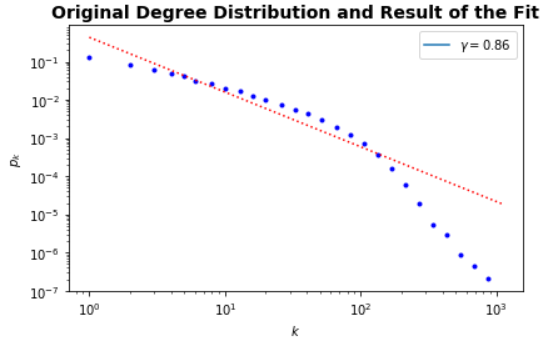
\includegraphics[width=0.9\linewidth]{images/problem43_degree_distribution.png}
		\caption{Real and fitted degree distribution of facebook links.}
		\label{distribution}
	\end{figure}
\end{enumerate}
